\documentclass[english]{beamer}
\usepackage[utf8]{inputenc}
\usepackage[T1]{fontenc}
\usepackage{babel}
\title{A Title}
\date{\today}
\author[Surname]{Author}
\subtitle{A Subtitle}
\usepackage{enumitem}
\usepackage{anyfontsize}

\usetheme{cleancolour}

% define new enum
\newenvironment{citemize}{\begin{itemize}[label={}]\Large\setlength\itemsep{1cm}\raggedright}{\end{itemize}}

\begin{document}

\titleframe

\fullScreenPicture{height=\paperheight}{figures/full-screen.jpg}

\tocframe

\section[Small description]{Section 1}

\begin{frame} 
\frametitle{Section 1} 
\begin{citemize}
\item Title of slide 1
\item Title of slide 2
\item Title of slide 3
\end{citemize}
\end{frame}

\begin{frame} 
\frametitle{Title of slide 1 } 
Some text and illustrations to support this portion of the talk. Notice the nice colour on the side!
\end{frame}

\tocframe

\section[Another small description]{Section 2}

\begin{frame}{LEDs, buttons and speaker provide user interface}
\centering
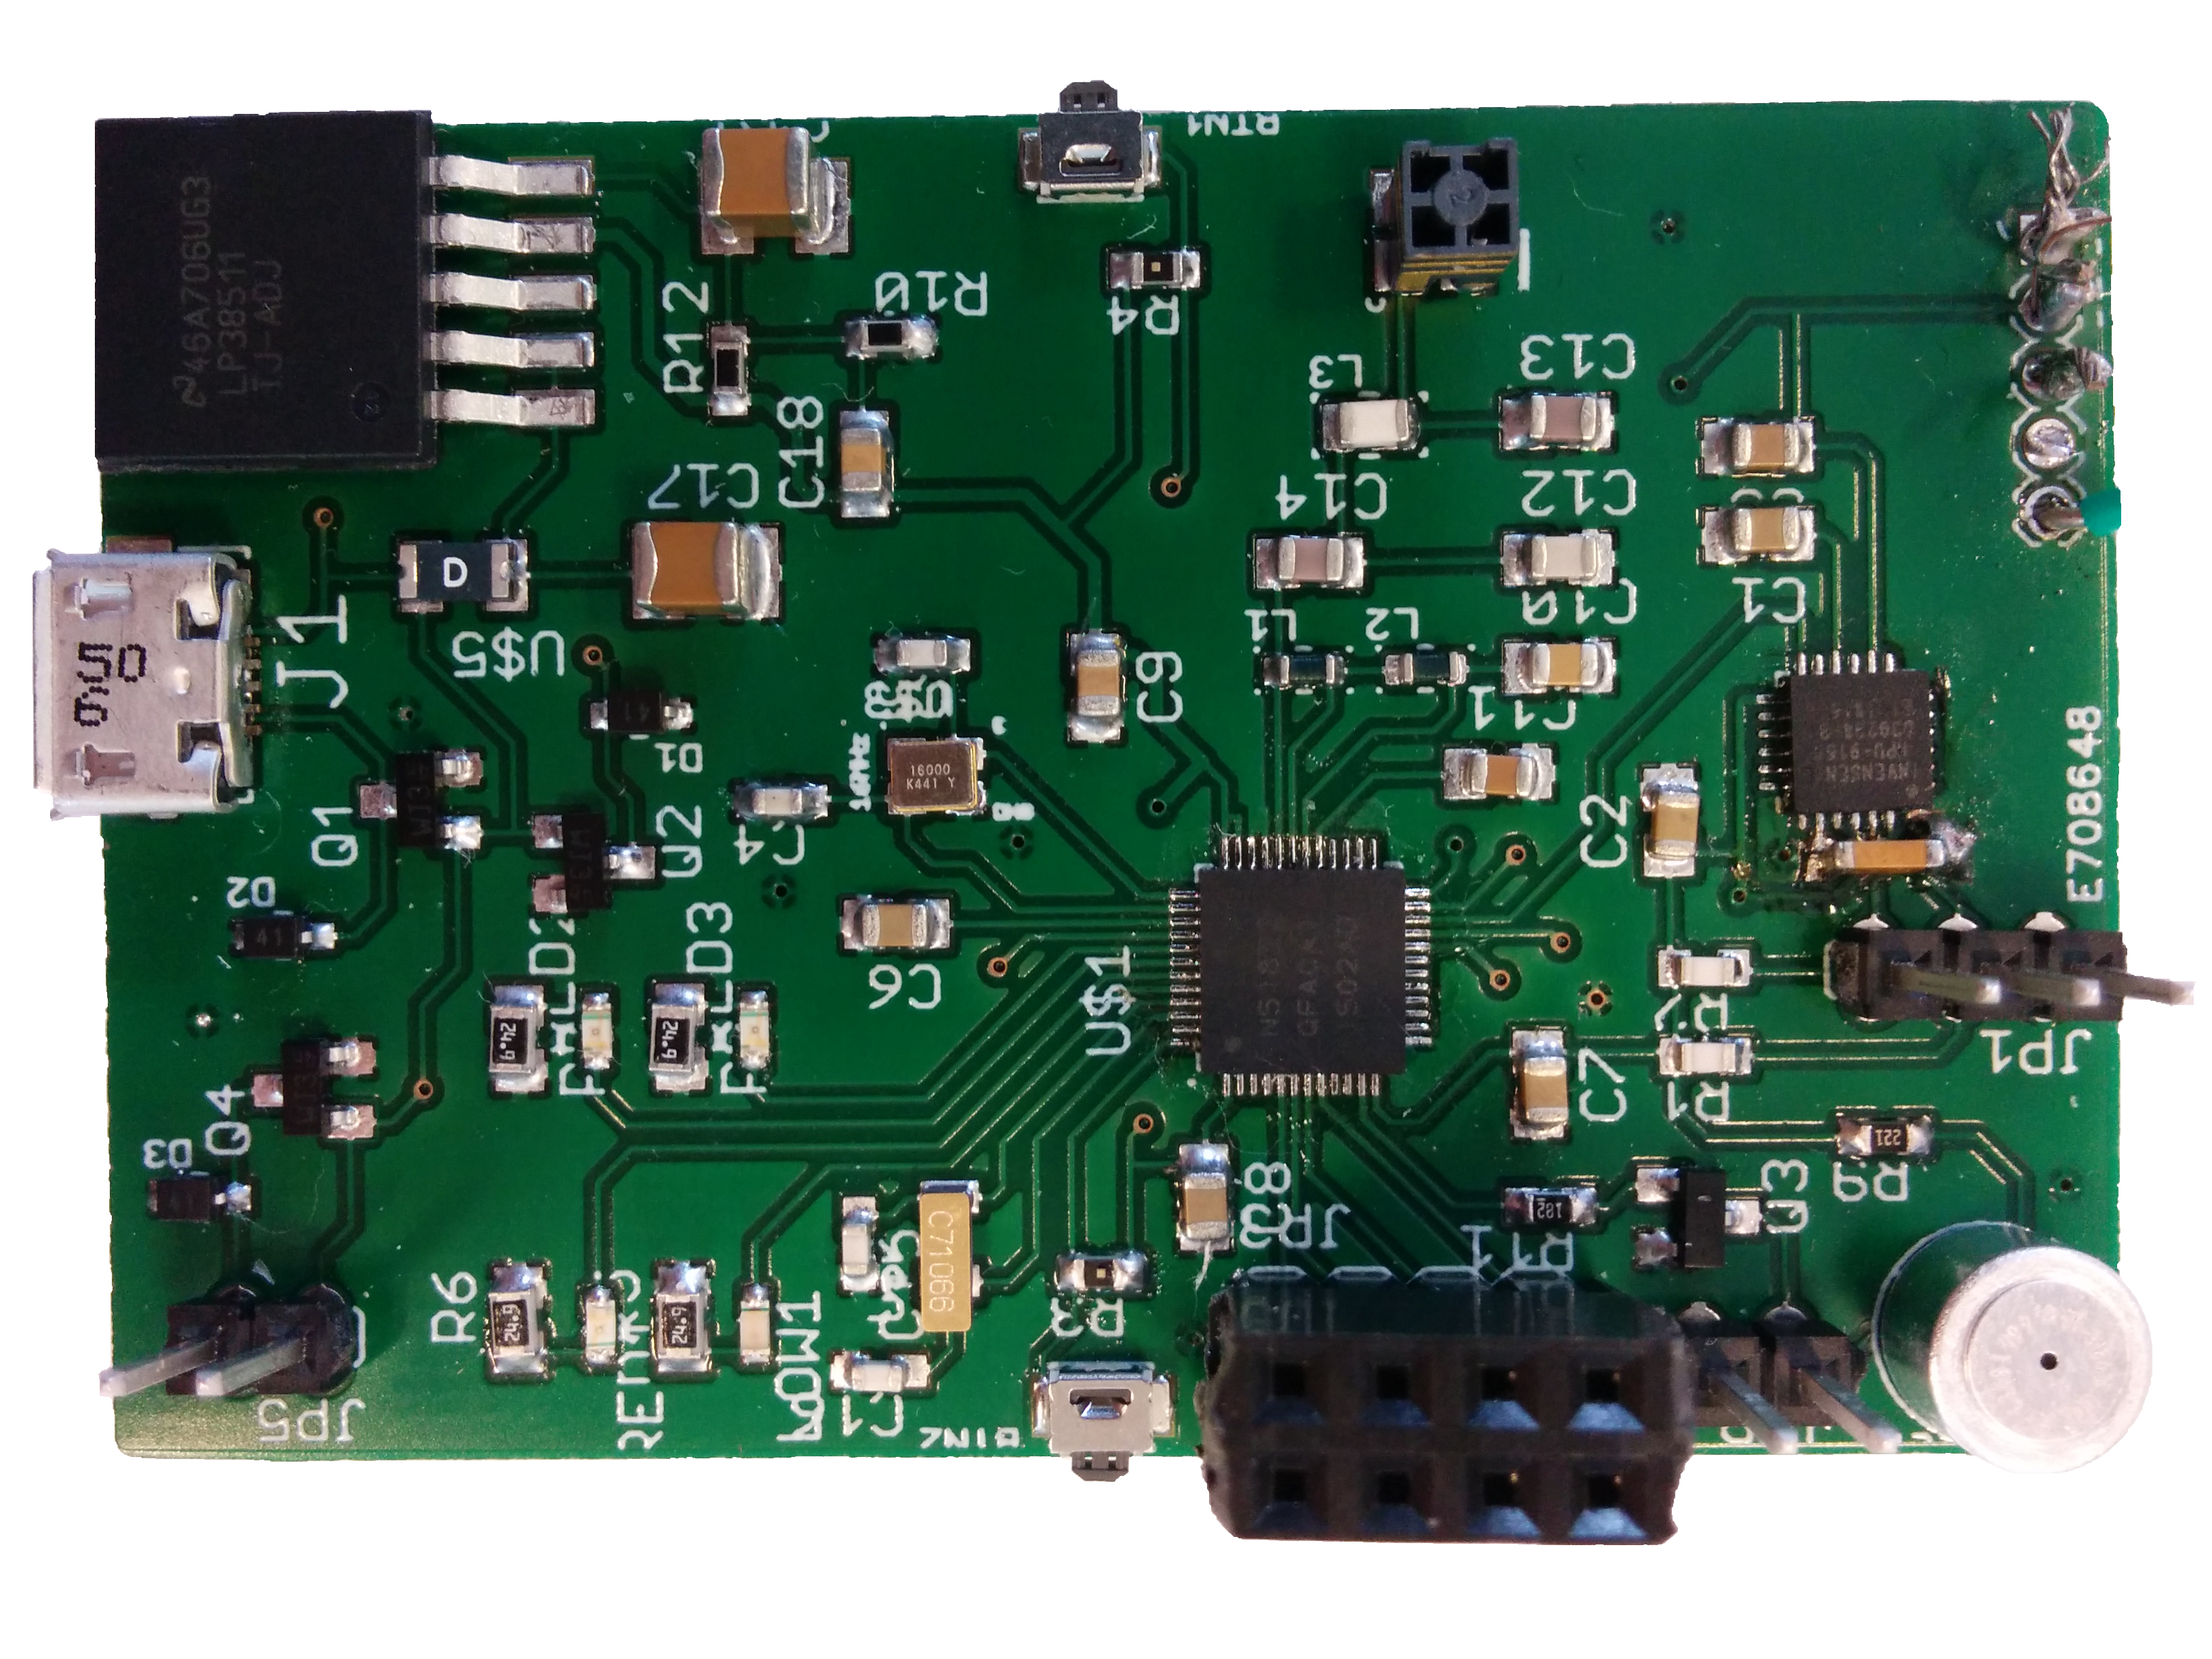
\includegraphics[width=\linewidth,height=0.8\textheight,keepaspectratio]{figures/PCB.jpg}
\end{frame}

\tocframe

\begin{frame}{Measurements}
\centering
\includegraphics[width=\linewidth,height=0.8\textheight,keepaspectratio]{figures/dist1.png}
\end{frame}

\tocframe

\begin{frame}{Conclusion}
A well constructed conclusion to wrap up the presentation. Possibly refer back to the introduction (to close the circle). 
\end{frame}

\fullScreenPicture{height=\paperheight}{figures/full-screen.jpg}

\end{document}